\begin{pastexam}[label={px:ntu-108-bime-ds-04}]{臺大生機所 108 學年度 第 4 題}
（問答＋設計）

(15\%) If you are given two traversal sequences, can you construct the binary tree? Write a pseudo
code to implement your answer. Please return the root of the binary tree as the output.
\end{pastexam}

\begin{pastsoln}
\textbf{答案：要看是哪兩種。} 假設節點的鍵值互不相同（有重複時連中序也分不出誰是誰）。
\begin{itemize}
\item \textbf{中序＋前序}、\textbf{中序＋後序}：可以，而且樹唯一（資結書第~7.4~節定理~7.4）。
前序的第一個（後序的最後一個）是根；在中序裡找到根，左邊是左子樹、右邊是右子樹，兩邊的大小
決定前序（後序）要怎麼切，再對兩邊遞迴。
\item \textbf{前序＋後序}：一般不行。 反例：根 $A$ 只有一個子節點 $B$，不論 $B$ 是左孩子還是
右孩子，前序都是 $A\,B$、後序都是 $B\,A$。 只有在每個內部節點都恰有兩個孩子（full binary
tree）時才唯一（資結書定理~7.5）。
\end{itemize}
所以要建樹，兩個序列裡必須有一個是中序。 下面寫「中序＋前序」，就是資結書虛擬碼~7.5。

\begin{pseudo}{由前序和中序建樹，回傳根}
\Function{Build-Tree}{$\mathit{pre}[1..n], \mathit{in}[1..n]$}
    \For{$j \gets 1$ \To $n$}
        \State $\mathit{pos}[\mathit{in}[j]] \gets j$ \Comment{每個鍵值在中序的位置}
    \EndFor
    \State \Return \Call{Build}{$1, 1, n$}
\EndFunction
\Function{Build}{$i, j, m$} \Comment{$\mathit{pre}[i..i{+}m{-}1]$ 和 $\mathit{in}[j..j{+}m{-}1]$ 是同一棵子樹}
    \If{$m = 0$}
        \State \Return \NIL
    \EndIf
    \State $k \gets \mathit{pos}[\mathit{pre}[i]]$ \Comment{根在中序的位置}
    \State $\ell \gets k - j$ \Comment{左子樹的節點數}
    \State 配置新節點 $x$，$x.\mathit{key} \gets \mathit{pre}[i]$
    \State $x.\mathit{left} \gets$ \Call{Build}{$i + 1, j, \ell$}
    \State $x.\mathit{right} \gets$ \Call{Build}{$i + 1 + \ell, k + 1, m - 1 - \ell$}
    \State \Return $x$
\EndFunction
\end{pseudo}
給的是中序＋後序時，第 8、10 行的根改成 $\mathit{post}[i + m - 1]$（子樹的最後一個），第 11 行
左子樹的後序從 $i$ 開始、第 12 行右子樹的後序從 $i + \ell$ 開始，其餘不變。

\textbf{追蹤}，前序 $A\,B\,D\,E\,C\,F$、中序 $D\,B\,E\,A\,F\,C$，每一列處理一棵子樹：
\begin{center}
\begin{tabular}{llcll}
\toprule
子樹的前序 & 子樹的中序 & 根 & 左子樹（中序） & 右子樹（中序） \\
\midrule
$ABDECF$ & $DBE\,|\,A\,|\,FC$ & $A$ & $DBE$ & $FC$ \\
$BDE$ & $D\,|\,B\,|\,E$ & $B$ & $D$ & $E$ \\
$CF$ & $F\,|\,C\,|$ & $C$ & $F$ & 空 \\
\bottomrule
\end{tabular}
\qquad
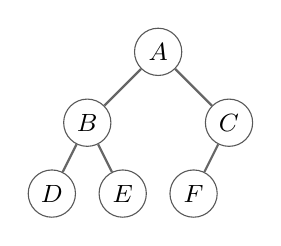
\begin{tikzpicture}[baseline=(r.center),
    btn/.style={circle, draw=black!65, line width=0.4pt, minimum size=6mm, inner sep=0pt, font=\small},
    level distance=9mm, edge from parent/.style={draw=black!60, thick},
    level 1/.style={sibling distance=18mm}, level 2/.style={sibling distance=9mm}]
\node[btn] (r) {$A$}
    child {node[btn] {$B$} child {node[btn] {$D$}} child {node[btn] {$E$}}}
    child {node[btn] {$C$} child {node[btn] {$F$}} child[missing]};
\end{tikzpicture}
\end{center}
建出來的樹後序是 $D\,E\,B\,F\,C\,A$，用中序＋後序的版本也會建出同一棵。

\textbf{正確性}（對子樹大小 $m$ 歸納）。 $m = 0$ 回傳空樹，對。 $m \ge 1$ 時，前序的第一個
$\mathit{pre}[i]$ 是根；中序是「左子樹、根、右子樹」，根在中序第 $k$ 格，所以左子樹有
$\ell = k - j$ 個節點，中序是 $\mathit{in}[j..k-1]$，右子樹是 $\mathit{in}[k+1..j+m-1]$。 前序是
「根、左子樹、右子樹」，所以左子樹的前序是 $\mathit{pre}[i+1..i+\ell]$，右子樹是
$\mathit{pre}[i+1+\ell..i+m-1]$。 兩次遞迴的大小都小於 $m$，由歸納假設建對，接上根就是整棵樹。

\textbf{複雜度。} 每個節點建一次，用 $\mathit{pos}$ 表找根是 $\Theta(1)$，總時間 $\Theta(n)$
（鍵值範圍大時 $\mathit{pos}$ 用雜湊表）。 不建 $\mathit{pos}$、每次在中序裡從頭找根的話，最壞
（歪斜的樹）是 $\Theta(n^2)$。
\end{pastsoln}
